\documentclass[xcolor={table}]{beamer}

% Packages
\usepackage[brazil]{babel}	
\usepackage[utf8]{inputenc}
\usepackage[T1]{fontenc}
\usepackage[scaled]{helvet}
\usepackage{amsthm}
\usepackage{ragged2e}
\usepackage{subfig}
\usepackage[table]{xcolor}
\usepackage{multicol}
\usepackage{multirow}
\usepackage{fancyvrb}
\usepackage{verbatim}
\usepackage{minted}

% Configuration for packages
\usemintedstyle{bw}

% Theme
\usetheme{Execushares}

% Title page configuration
\title{Laborator I: Introducere}
\subtitle{}
\author{Iosif George-Andrei}
\setcounter{showSlideNumbers}{1}

\begin{document}

    % Title page
    \setcounter{showProgressBar}{0}
	\setcounter{showSlideNumbers}{0}
	\frame{\titlepage}

    % Table of content
	\begin{frame}
		\frametitle{Tabelă de Conținut}\pause
		\begin{enumerate}[<+->]
			\item BinExpLabs 101
			\item Noțiuni Introductive
			\item Exploatarea Executabilelor
			\item Instrumente
		\end{enumerate}
	\end{frame}

    % First section
	\setcounter{framenumber}{0}
	\setcounter{showProgressBar}{1}
	\setcounter{showSlideNumbers}{1}
	\section{BinExpLabs 101}

	\begin{frame}
		\frametitle{Notare}\pause
		\begin{enumerate}[<+->]
			\item Laboratoare ($ 50\% $ din notă)
			    \begin{itemize}
			        \item Rezolvarea în timpul laboratorului
			        \item Participarea la \textit{quiz}-uri
			    \end{itemize}
			\item Temă de casă ($ 50\% $ din notă)
			    \begin{itemize}
			        \item Detalierea rezolvării
			        \item Fără plagiat
			    \end{itemize}
		\end{enumerate}
	\end{frame}
	
	\begin{frame}
		\frametitle{Regulile Jocului}\pause
		\begin{itemize}[<+->]
			\item Atenție în cadrul laboratoarelor
			\item Respect reciproc
		\end{itemize}
	\end{frame}
	
	\begin{frame}
		\frametitle{\textit{Must-have}}\pause
		\begin{itemize}[<+->]
		    \item Resurse
		        \begin{itemize}
    				\item Mașină virtuală cu Linux
    				\item Python 3 cu librăria \mintinline{bash}{pwntools}
    				\item Ghidra
    				\item PEDA
		        \end{itemize}
		\end{itemize}
	\end{frame}
	
	\begin{frame}
		\frametitle{\textit{Nice to Have}}\pause
		\begin{itemize}[<+->]
			\item Cunoștințe de limbaj de asamblare
			\item Cunoștințe despre sisteme de operare
			\item Experiență cu Linux
			\item Experiență cu Python 3
		\end{itemize}
	\end{frame}
	
	 % Second section
	\section{Noțiuni Introductive}
	
	\begin{frame}
		\frametitle{Procese. Executabile}\pause
		\begin{itemize}[<+->]
		    \item \textbf{Proces}: Set de instrucțiuni ce sunt grupate pentru a fi \textbf{executate} pe procesor, în cadrul \textbf{sistemului de operare} gazdă, cu scopul de a transforma \textbf{date de intrare} în \textbf{date de ieșire}.
			\item \textbf{Executabil}: Fișier care încapsulează instrucțiuni ce trebuiesc executate de procesor și pe baza căruia este creat un proces. Numit și binar.
			\item Cele mai comune \textbf{formate}
			    \begin{itemize}
        			\item Portable Executable (abreviat PE, specific Windows)
        			\item \textbf{Executable and Linkable Format} (abreviat ELF, specific Unix)
        		\end{itemize}
		\end{itemize}
	\end{frame}
	
	\begin{frame}
		\frametitle{Formatul ELF}\pause
        \centering
        \mintinline{bash}{sketch();}
	\end{frame}
	
	\begin{frame}
		\frametitle{Memoria unui Proces}\pause
		\centering
        \mintinline{bash}{sketch();}
	\end{frame}
	
	\begin{frame}
		\frametitle{Stiva unui Proces}\pause
		\centering
        \mintinline{bash}{sketch();}
	\end{frame}
	
	 % Third section
	\section{Exploatarea Executabilelor}
	
	\begin{frame}
		\frametitle{Terminologie}\pause
		\begin{itemize}[<+->]
		    \item \textbf{Vulnerabilitate}: Slăbiciune a unui sistem informatic, ce poate provoca o funcționare incorectă a lui.
			\item \textbf{Exploatare}: Atacarea cu succes a unui sistem informatic, prin intermediul unei vulnerabilități.
		    \item \textbf{Exploatarea Executabilelor}: Provocarea de către un atacator a execuției incorecte a unui executabil.
		\end{itemize}
	\end{frame}
	
	\begin{frame}
		\frametitle{Suprafața de Atac}\pause
		\begin{itemize}[<+->]
		    \item \textbf{Set de puncte} (numite vectori de atac) de la marginea unui sistem informatic  pe care \textbf{un atacator le poate folosi} pentru a interacționa cu el (obținerea accesului, extragerea datelor, perturbarea funcționării).
		    \item Vectori uzuali de atac
    		    \begin{itemize}
        		    \item \mintinline{bash}{stdin}
        		    \item Argumente
        		    \item Variabile de mediu
        		    \item Fișiere (de configurație, baze de date)
        		    \item Întreruperi
        		    \item Dispozitive
    		    \end{itemize}
		\end{itemize}
	\end{frame}
	
	\begin{frame}
		\frametitle{Motivație}\pause
		\begin{itemize}[<+->]
		    \item Înțelegerea \textbf{mentalității de atacator}
		    \item \textbf{\textit{Bug bounty}}
    		    \begin{itemize}
    		        \item CVE-2019-5790, ca \textit{integer overflow} în Google Chrome, ce permitea execuția de cod de la distanță
    		    \end{itemize}
		    \item \textbf{\textit{Zero days}}
		        \begin{itemize}
    		        \item \textit{Marketplaces}, precum Zerodium
    		        \item Utilizarea în atacuri avansate, precum Stuxnet
    		    \end{itemize}
		\end{itemize}
	\end{frame}
	
	% Forth section
	\section{Instrumente}
	
	\begin{frame}
		\frametitle{Pur Statice}\pause
		\begin{itemize}[<+->]
		    \item \textbf{\mintinline{bash}{strings}}: Extragerea șirurilor de caractere printabile din fișiere.
		    \item \textbf{\mintinline{bash}{nm}}: Extragerea simbolurilor din fișierele obiect (atât executabile, cât și librării).
		    \item \textbf{\mintinline{bash}{ldd}}: Extragerea dependințelor către librării dinamice.
		    \item \textbf{\mintinline{bash}{objdump}}: Extrage informații din fișiere obiect. Poate fi folosit pentru dezasamblare.
		    \item \textbf{\mintinline{bash}{Ghidra}}: Instrument pentru inginerie inversă, cu funcționalități de dezasamblare și decompilare.
	    \end{itemize}
	\end{frame}
	
	\begin{frame}
		\frametitle{Pur Dinamice}\pause
		\begin{itemize}[<+->]
		    \item \textbf{\mintinline{bash}{ltrace}}: Interceptarea apelurilor către librării dinamice.
		    \item \textbf{\mintinline{bash}{strace}}: Interceptarea apelurilor de sistem.
		    \item \textbf{\mintinline{bash}{netstat}}: Oferă detalii despre rețelistică, util pentru urmărirea conexiunilor efectuate.
		    \item \textbf{\mintinline{bash}{gdb}}: Depanează programe, putând fi folosit împreună cu \textbf{PEDA}.
	    \end{itemize}
	\end{frame}
	
	\begin{frame}
		\frametitle{Altele}\pause
		\begin{itemize}[<+->]
		    \item \textbf{\mintinline{bash}{pwntools}}: Librărie Python3 ce ușurează exploatarea programelor
		    \item \textbf{\mintinline{bash}{man}}: Interfață pentru manualele comenzilor.
	    \end{itemize}
	\end{frame}
	
	% Fifth section
	\section{Exerciții}
	
	\begin{frame}
		\frametitle{Recomandări}\pause
		\begin{itemize}[<+->]
		    \item Folosiți comanda \mintinline{bash}{man} pentru a primi ajutor la rularea anumitor comenzi.
		    \item Folosiți \href{https://docs.pwntools.com/en/stable/}{documentația \mintinline{bash}{pwntools}} pentru a identifica metodele de care aveți nevoie.
	    \end{itemize}
	\end{frame}
	
    % Sixth section
	\section{Recapitulare}
	
	\begin{frame}
		\frametitle{Recapitulare}\pause
		\begin{figure}
            \centering
            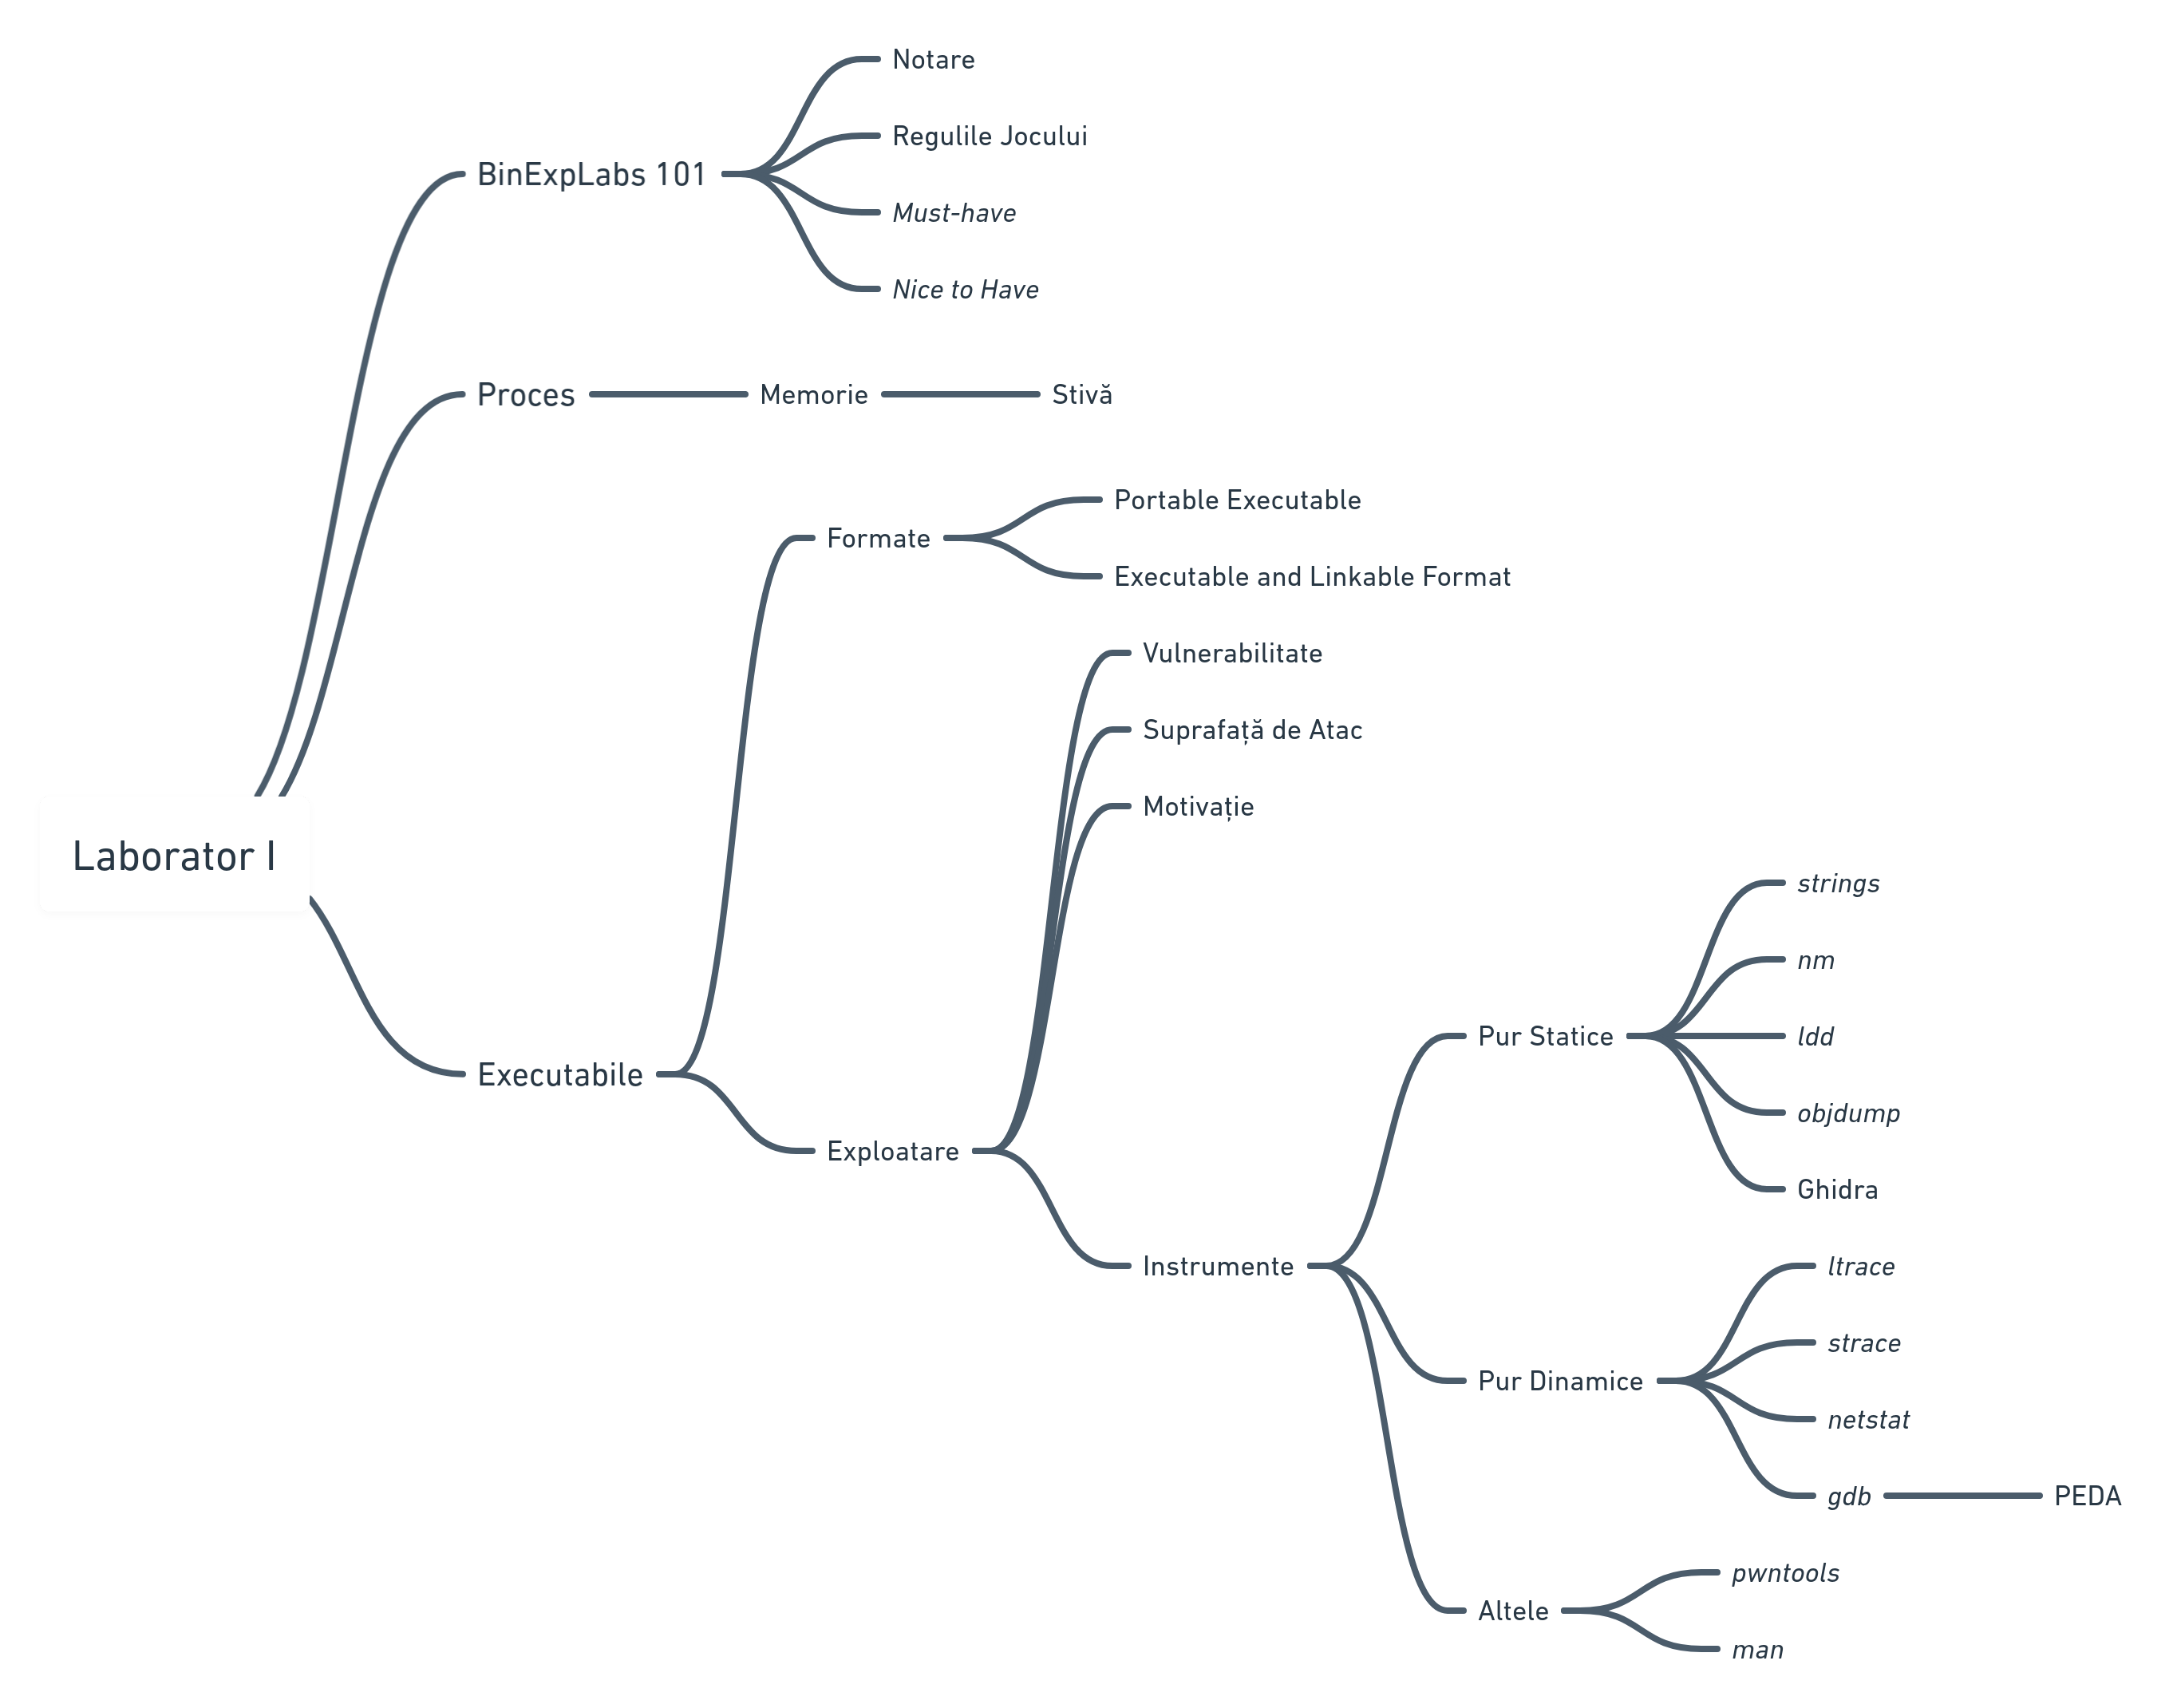
\includegraphics[width=9cm]{images/recap.png}
        \end{figure}
	\end{frame}

\end{document}